\section{Transformador}
A menudo se utiliza un transformador para acoplar el voltaje de entrada de ca
proveniente de la fuente al rectificador. El acoplamiento por transformador
ofrece dos ventajas:

\begin{itemize}
    \item Permite que la fuente de voltaje se reduzca como sea necesario.
    \item La fuente de ca se aísla eléctricamente del rectificador, con lo que
        se evita el peligro de choques eléctricos en el circuito del
        secundario \cite{Floyd}.
\end{itemize}

Se utilizará un transformador de $220[\text{V}]$ a $12[\text{V}]$ con derivación
central de $1[\text{A}]$, con los voltajes descritos en la
\textbf{figura~\ref{circuito01}}.

\begin{figure}[!h]
\centering
\includegraphics[scale=1]{diagramas/01.transformador.eps}
\caption{Voltajes de entrada y salida del transformador.}
\label{circuito01}
\end{figure}

\subsection{Simulación}
Se utilizó el software \emph{Quite Universal Circuit Simulator.} versión 23.3.1
para la simulación del transformador, este puede verse en la
\textbf{figura~\ref{simulacion01}}.

\begin{figure}[!h]
\centering
\includegraphics[scale=0.75]{simulacion/01.transformador.eps}
\caption{Simulación del transformador de $220[\text{V}]$ a $12[\text{V}]$.}
\label{simulacion01}
\end{figure}

\subsection{Laboratorio}
Para los experimentos se utilizó el transformador mostrado en la
\textbf{figura~\ref{laboratorio01}}.

\begin{figure}[!h]
\centering
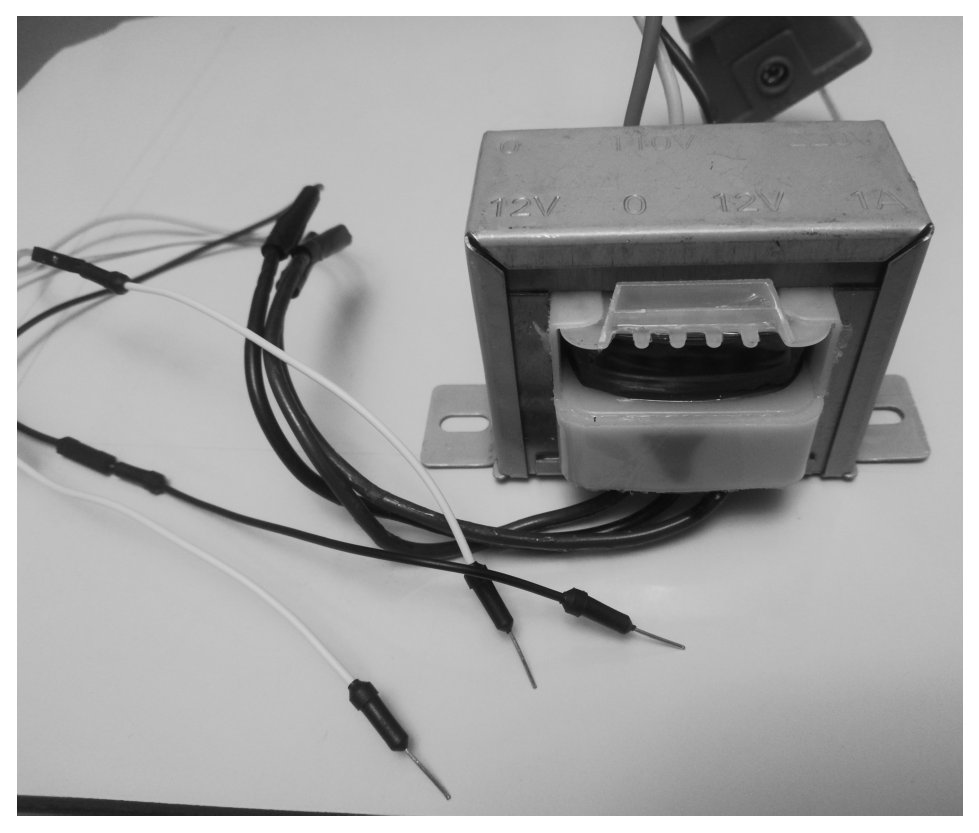
\includegraphics[scale=0.28]{fotos/01.transformador1.eps}
\caption{Transformador con derivación central.}
\label{laboratorio01}
\end{figure}

El transformador puede usarse para disponer de una salida de $12[\text{V}]$ o
una de $24[\text{V}]$, segun se utilizen dos de sus tres terminales, como puede
verse en la \textbf{figura~\ref{laboratorio02}} y la
\textbf{figura~\ref{laboratorio03}} respectivamente.

\begin{figure}[!h]
\centering
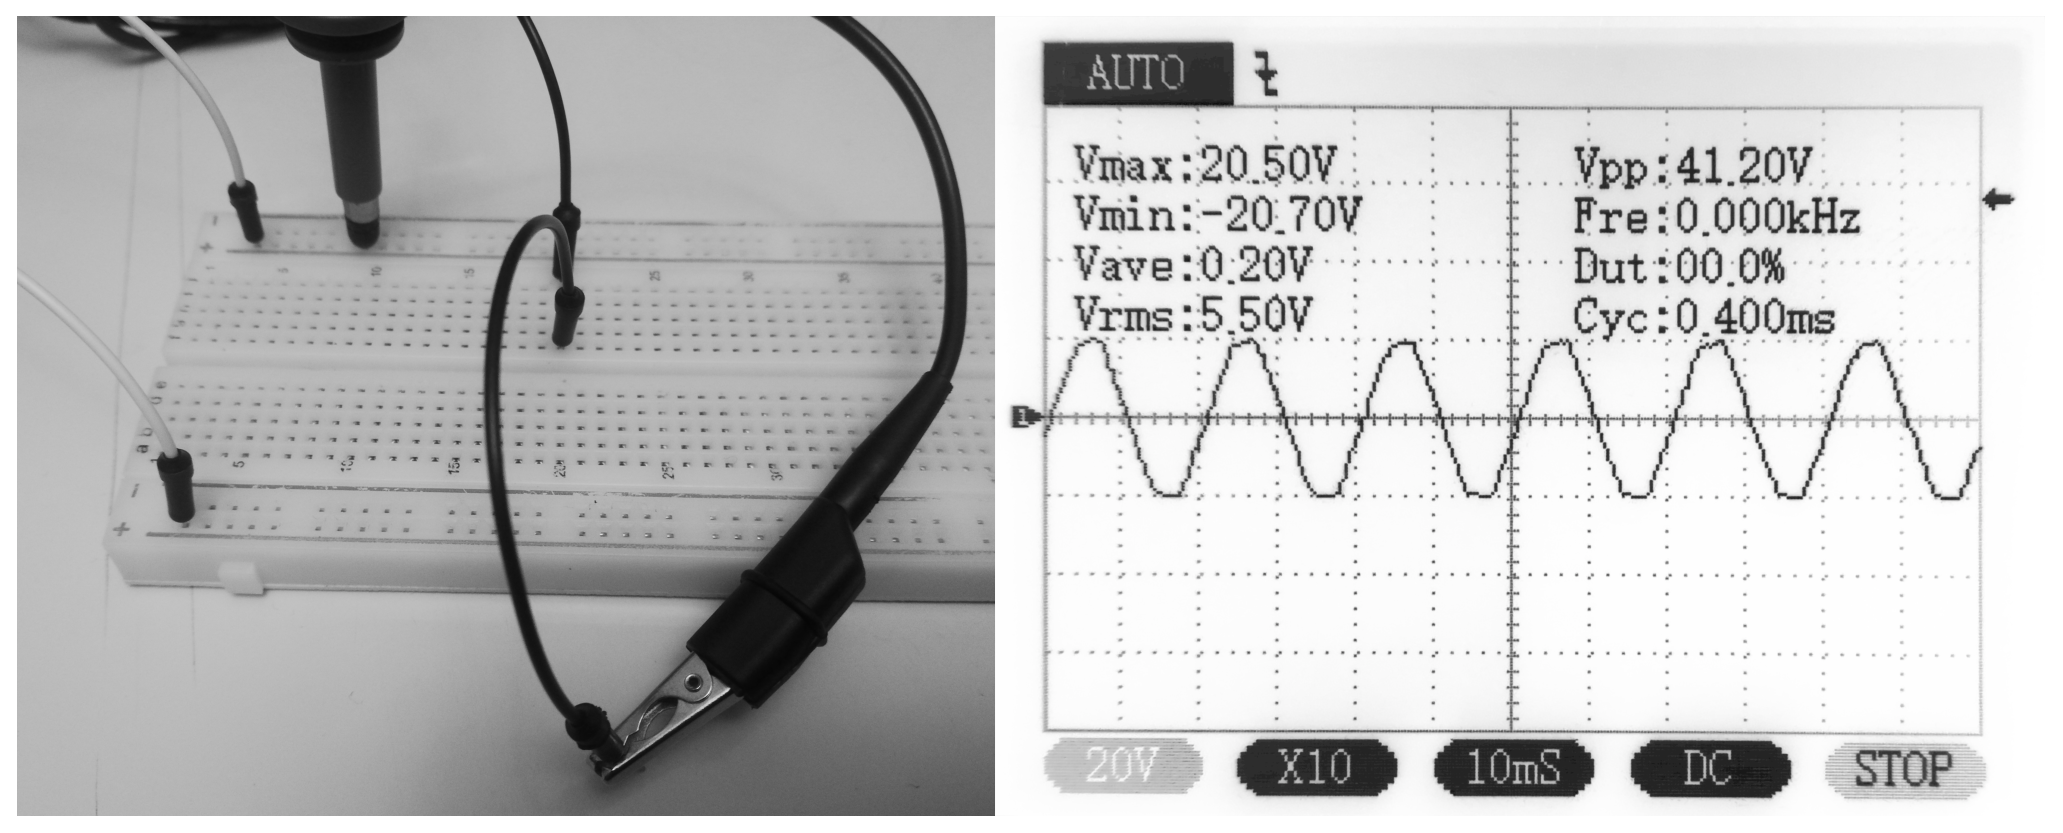
\includegraphics[scale=0.28]{fotos/01.transformador2.eps}
\caption{Señal de salida del transformador a $12[\text{V}]$.}
\label{laboratorio02}
\end{figure}

\begin{figure}[!h]
\centering
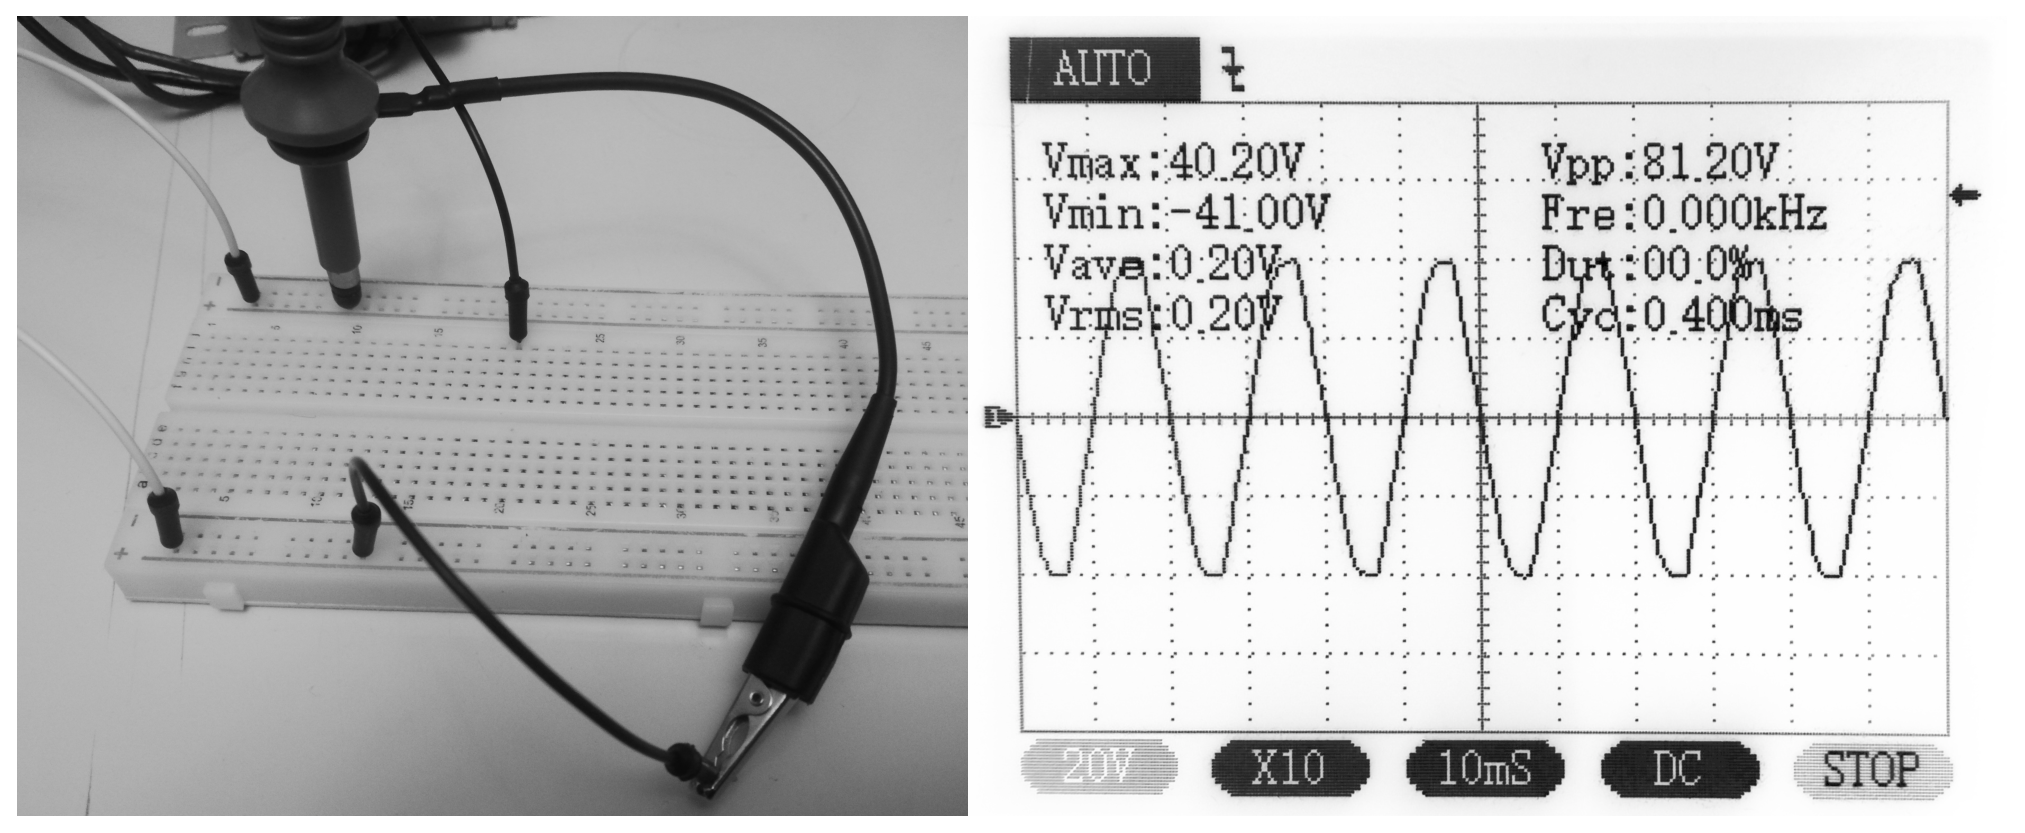
\includegraphics[scale=0.28]{fotos/01.transformador3.eps}
\caption{Señal de salida del transformador a $24[\text{V}]$.}
\label{laboratorio03}
\end{figure}

